\chapter{Path planning with respect to the end effector}

As of now, we have a fast inverse kinematics algorithm, which allows us to compute joint positions, given the \textit{end effector} position of the manipulator. If we can find a suitable path for the \textit{end effector} to follow, we can discretize it into small steps and use our extension of FABRIK to compute incremental changes along the path for the rest of the manipulator.

Although we have a myriad of algorithms to deal with the 3-dimensional path planning problem, the task is not as simple as our initial example of a robot that can move in any direction; we need to find paths that can be followed with the remainder of the manipulator.

This chapter goes through the process of designing such an algorithm for the task at hand.

\section{Grid based approach}

Recall that one of the successfull ways of applying this technique has been mentioned in~\cite{rrt_fabrik}, where the authors expand a RRT and compute FABRIK at every node. However, our extended FABRIK is too slow to compute for every point in the workspace; hence, we want to limit the amount of times we run the algorithm to lower hundreds.

Therefore, we want to find paths that lead to a solution with a high probability, and only compute FABRIK on points on this path. In case FABRIK fails on this path, for instance due to the manipulator being too short to get around an obstacle, we want to fall back and look for a different path.

Out of the three basic approaches, our go-to are the shortest path in a graph algorithms. As mentioned earlier, gradient based methods are not helpful due to the local minima problem and only generating a single possible path. Similarly, one of the weaknesses of the RRT algorithm is that it only finds a single path, and trying to generate edges between all possible nodes to find multiple paths would be computationally infeasible.

As a baseline for discretization of space, a grid based approach was tested out. This is not optimal for multiple reasons, but it is implementationally simple, allows us to analyze the procedure, and explore further extensions. Note that while the original Djikstra's algorithm works with weighted edges, in this case, we are assigning weights to vertices. Any edge that leads to a given vertex is treated as if it has the weight of the vertex during the shortest path algorithm.

Points on the grid were spaced out at half the size of a single joint, striking a balance between not generating too many points and making the shortest path algorithm too slow, and still being able to explore \textit{most} viable paths\footnote{This claim no longer holds if we consider many tiny obstacles, but the assumption that static objects are of comparable size to the joints of the manipulator is fairly reasonable. Spacing at half the joints' size means that if the manipulator fits in a space between obstacles, it will often be found.}.

The advantage of this representation is that we can weigh the points on the grid to influence which paths will be evaluated as optimal. We borrow the idea from the Artificial Potential Field algorithms, and give more weight to areas that surround an obstacle.

Points on the grid that are occupied by an obstacle are assigned an infinite weight, clearly no path can lead through them. In the area surrounding each obstacle, the weight will be high. Generally, we want the algorithm to choose paths further from obstacles, if possible. This follows the reasoning that we want to accomodate for the rest of the manipulator. If the path for the \textit{end effector} leads closely around obstacles, the chance that the remaining joints of the manipulator will fit is also lowered. However, while expensive, we want the paths close to obstacles to be evaluated as viable, since there may not be other options.

Each obstacle affects the surrounding area and raises the surrounding points on the grid based on how far they are. The total effect of obstacles is summed up; as a result, points between multiple obstacles are given a very high cost. A high cost between clusters of obstacles leads to the desired effect of preferring safer paths that avoid them altogether, though the path itself may be longer.

\begin{figure}
    \centering
    \begin{subfigure}{.3\textwidth}
      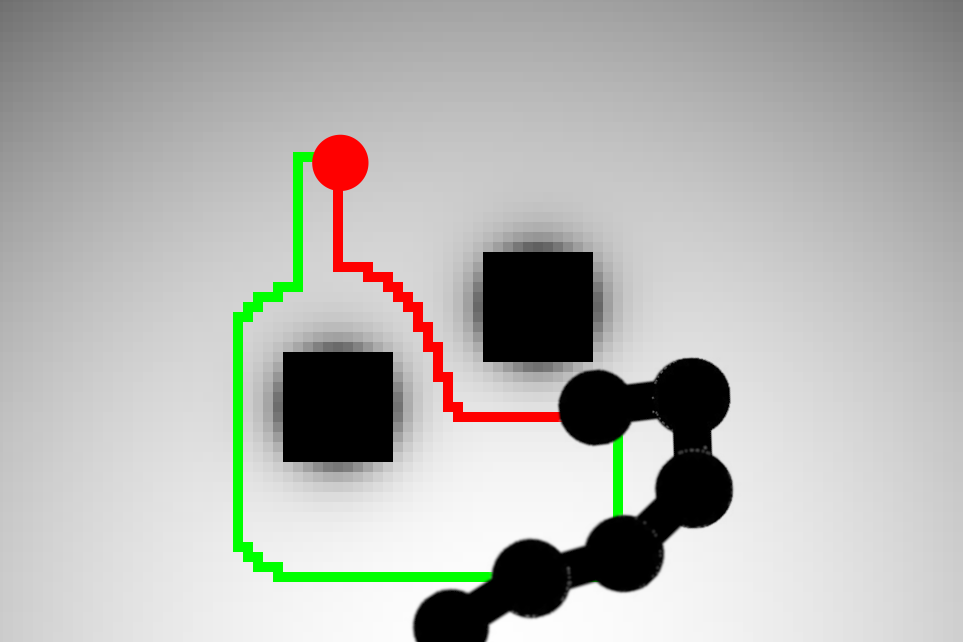
\includegraphics[width=0.99\textwidth]{manipulator_initial.png}
      \caption{Initial position of the manipulator, a target, and the first 2 paths found by the algorithm.}
    \end{subfigure}
    \begin{subfigure}{0.3\textwidth}
      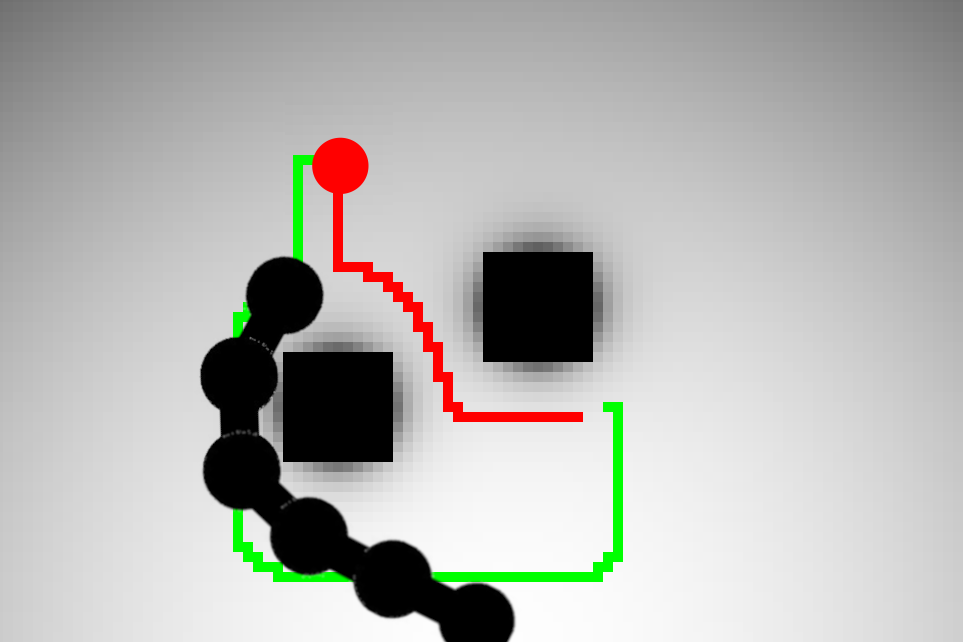
\includegraphics[width=0.99\textwidth]{manipulator_short.png}
      \caption{The careful path around obstacles does not lead to a solution, due to the manipulator being too short.}
    \end{subfigure}
    \begin{subfigure}{.3\textwidth}
      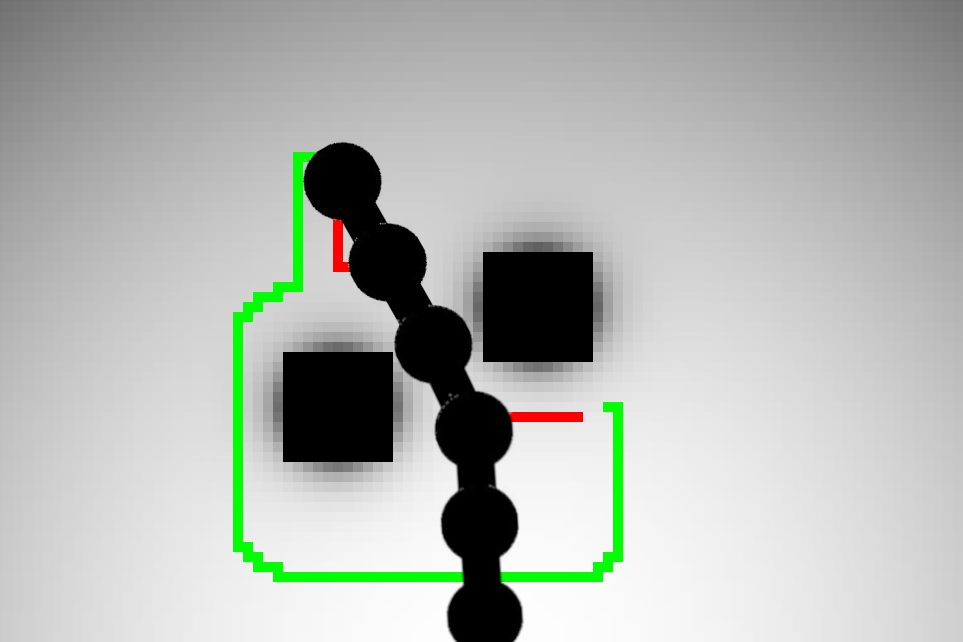
\includegraphics[width=0.99\textwidth]{manipulator_between.png}
      \caption{The viable path for the \textit{end effector} leads between the obstacles.}
    \end{subfigure}
    \caption{Illustration of the extended shortest path algorithm on a weighted grid. Black boxes represent obstacles, and the opacity of the background represents the cost of traversing over a given square.}\label{fig:paths}
\end{figure}

In effect, the algorithm works in the same fashion as APF, but does not suffer from local minima. If the first path we found is evaluated as wrong, the cost of points close to the found path is increased, and the algorithm looks for a new path in the modified graph. If, for instance, there are two obstacles and the only viable way to reach the target leads through them, paths around them may be evaluated as better at first. Trying to reproduce the path with FABRIK will fail due to the manipulator being too short, the cost near the found path is raised, and eventually the path between them is found. The idea is visualized in Figure~\ref{fig:paths}.

\begin{wrapfigure}{r}{0.4\textwidth}
  \centering
  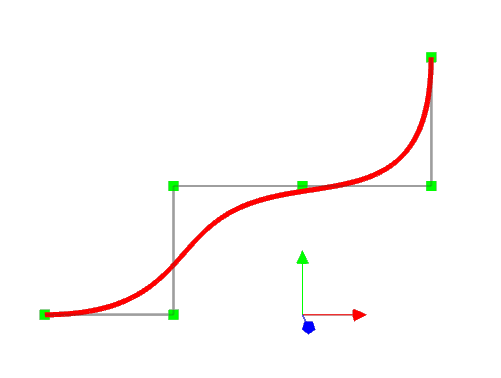
\includegraphics[width=0.4\textwidth]{nurbs_grid.png}
  \caption{B-splines can generate a smooth path from points on a grid (visualized using~\cite{nurbs_vis}).}
\end{wrapfigure}

The first obvious drawback of the algorithm is how rugged the resulting paths are. Instead of exactly following the found path and making unnecessary back and forth motion, we want to interpolate the points in a smooth way. Generating a smooth path from a set of points on the grid can be accomplished using B-splines~\cite{nurbs}.

B-splines, also known as basis splines, are piecewise polynomial functions used to generate smooth lines or shapes using a simple polynomial function and a set of control points.
To construct a B-spline, we need:

\begin{itemize}
\item A basis polynomial function given by its \textbf{order}. The order of the function determines how many nearby control points influence any the resulting points on the curve, and is always one more than the degree of the polynomial.
\item Sequence of \textbf{control points}. Control points determine the shape of the curve. Each point on the curve is determined as an interpolation between the nearby control points, using the sum of our basis functions for each of the points.
\item Sequence of \textbf{knots}. Knots are numbers in nondecreasing order, which determine where and how the control points affect the curve. The number of knots is always equal to the number of control points + the order of the curve. For trajectory generation, we can imagine the knot parameter as time. Then, we have a direct mapping of time to the position; knots specify by which control points the point will be influenced, and the ratio between the knot values specifies how much.
\end{itemize}

In the most common generalization of B-splines, Non-rational uniform B-splines (NURBS), each control point is also associated with a specific \textbf{weight}. When considering uniform points on a grid, we can just assign the same weight to each point.

Contrary to interpolating with polynomials directly, B-splines don't generally go directly through the control points. Going through a specific point can be achieved with a knot of a multiplicity equal to the order, which are commonly at the beginning and end of the curve. Since the curve order specifies how many control points influence each point, a lower curve order leads to curves closer to the control points, while a higher one can produce smoother paths overall.

\begin{figure}
  \centering
  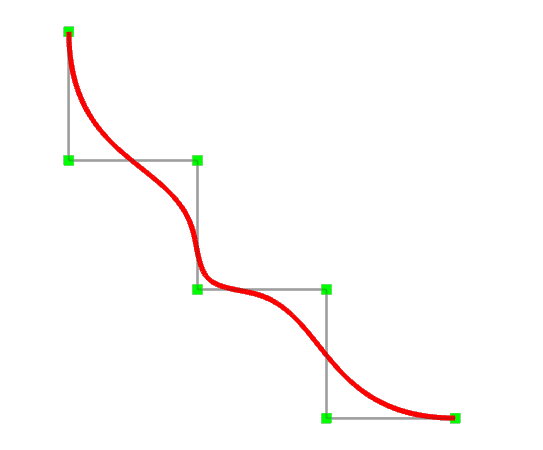
\includegraphics[width=0.5\textwidth]{nurbs_3.png}
  \caption{B-spline of order 4 with knots (0, 0, 0, 0, 0.4, 0.5, 0.6, 1, 1, 1, 1)}
\end{figure}

\begin{figure}
  \centering
  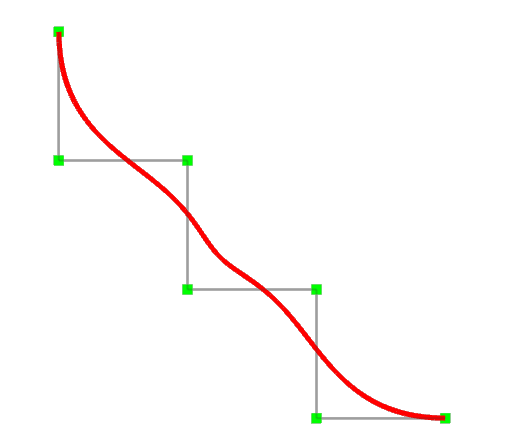
\includegraphics[width=0.5\textwidth]{nurbs_4.png}
  \caption{B-spline of order 5 with knots (0, 0, 0, 0, 0, 0.45, 0.55, 1, 1, 1, 1, 1)}
\end{figure}

To follow the curve with our inverse kinematics algorithm, we need to choose the size of our steps, get the value of the curve at the next time interval, and compute FABRIK starting at the current position. The only problem is that the curve only specifies the position, and the algorithm takes the entire transformation matrix as the input, including rotation. Hence, we need to look for ways to interpolate rotation as well.

In cases where the \textit{end effector} moves independently from the rest of the manipulator, Spherical linear interpolation (SLERP)~\cite{slerp} between the initial and target rotations is a suitable solution. The method uses quaternions to perform rotation at a constant velocity, resulting in a smooth motion.

Our case is a little different. In the case of RoFI manipulators, the rotation of the final module can influence how the entire manipulator needs to move, in order to accomodate for joint limits. Hence, we want to reach the target rotation as soon as possible. On the other hand, we need to consider that the target rotation may not be reachable immediately.

There isn't a single best way of choosing the angle interpolation, since the inputs and targets can vary wildly. A method that performs reasonably well is to interpolate euler angles of the initial \textit{end effector} position and target with a quadratic function rather than a linear one. The reasoning behind this is that early targets for FABRIK have to be close to the initial position, but the target rotation is reached quickly and we don't make unnecessary movements.

Now that we have all the pieces, we can run the algorithm and evaluate how good the paths found for the \textit{end effector} are.

\section{Optimising the manipulator trajectory}

Let us summarize the entire computation. Our input parameters are a model of the environment -- obstacles and a single manipulator, and a target for the manipulator's \textit{end effector} to reach. The algorithm does the following, in order:

\begin{enumerate}
\item The environment within which the manipulator exists is loaded, and a kinematic model of the manipulator is created.
\item An AABB tree for collision checking is created. The obstacles and joints are approximated via spheres and inserted into the tree.
\item A grid is created in the space the manipulator can move in. Each obstacle raises the cost on the surrounding points of the grid.
\item The shortest path on the weighted grid between the initial position of the \textit{end effector} and the target is found.
\item The found path is smoothed out by interpolating the found points on the grid with a B-spline.
\item The path is sampled at discrete points, and an extension of FABRIK is used to compute the joint parameters needed to reach each of the points.
\item If the path can be followed successfully, the movement is realised. Otherwise, if FABRIK fails to find viable positions on this trajectory, the algorithm falls back to step 4, adjusts the grid, and tries to find a different path.
\end{enumerate}

We can now demostrate initial results within a RoFI simulator. As a baseline, we will consider a manipulator that consists of a chain of 4 modules, linked via the $-Z$ connectors. Since such a manipulator has 12 degrees of freedom, previous state of the art algorithms -- which only scale up to 6 -- would clearly not be useful.

Let us start by visualizing the most basic case, to see if the produced motion is natural: the algorithm in a space with no obstacles.

\begin{figure}
  \centering
  \begin{minipage}{\textwidth}
    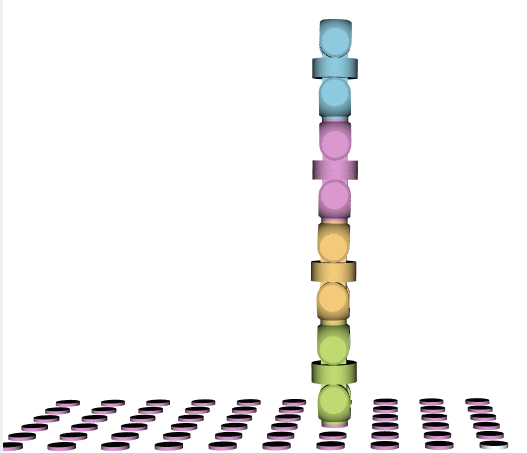
\includegraphics[width=0.3\textwidth]{sim1_0.png}
    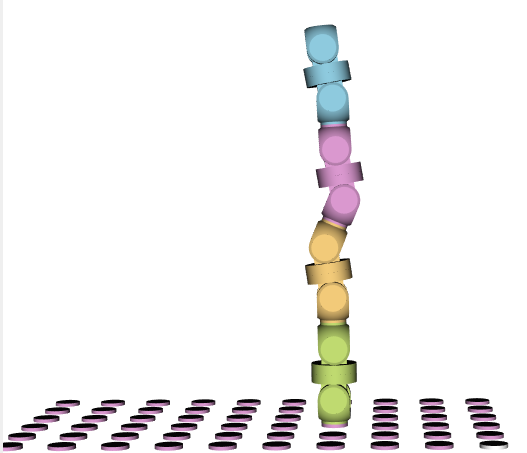
\includegraphics[width=0.3\textwidth]{sim1_1.png}
    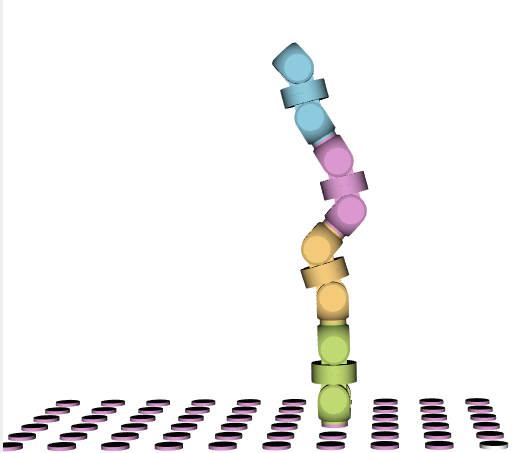
\includegraphics[width=0.3\textwidth]{sim1_2.png}

    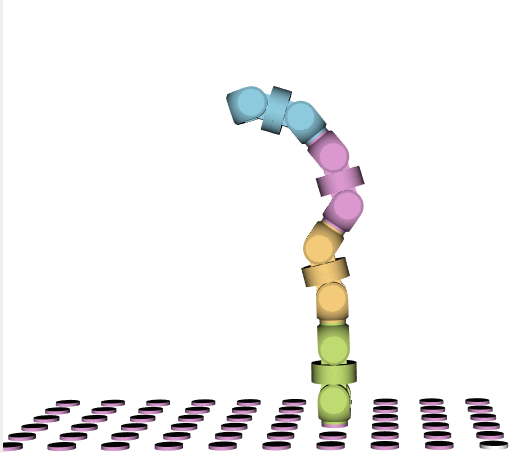
\includegraphics[width=0.3\textwidth]{sim1_3.png}
    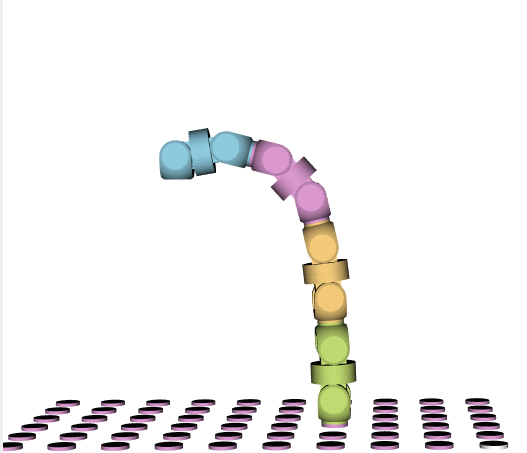
\includegraphics[width=0.3\textwidth]{sim1_4.png}
    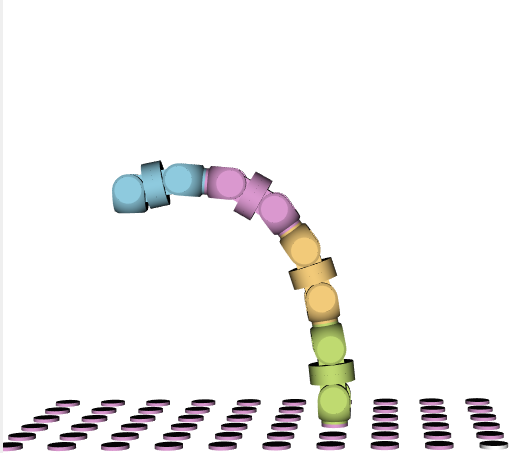
\includegraphics[width=0.3\textwidth]{sim1_5.png}
  \end{minipage}
  \caption{Our algorithm in a space with no obstacles.}\label{fig:sim1}
\end{figure}

As we can see in Figure~\ref{fig:sim1}, the found trajectory of the \textit{end effector} is smooth, including rotation. However, there is unnecessary motion before the manipulator adjusts itself into a straightened out position. Looking at the joints of the second and third module, they fold up during the algorithm, only to straighten themselves out again once the \textit{end effector} is closer to the target. We can reduce the amount of unnecessary motion by post-processing the calculated trajectory.

Note that our found trajectory is a sequence of positions for the manipulator. The whole reason behind creating this complex algorithm rather than simply using inverse kinematics is that we cannot trivially interpolate between the initial and final positions, due to the obstacles in the way. However, this doesn't hold for all the intermediate steps in the calculated sequence. For each pair of positions, we can, via simple interpolation, check if the steps between them can be skipped, and the transition can be made directly. As a result, we can avoid intermediate positions where the manipulator folds itself up, only to readjust later on.

For each position in the sequence, the post-processing algorithm checks how far in the sequence it can get via interpolating the current and following positions directly. The farthest the algorithm can get at any point becomes the next target, and the computed intermediate positions are discarded. The shortcutting algorithm can easily be expressed via the following pseudocode~\ref{alg:opt}.

\begin{algorithm}
 \SetKwInOut{Input}{input}\SetKwInOut{Output}{output}
 \Input{Sequence of manipulator positions $P[0..n]$}
 \Output{Sequence of manipulator positions $O[0..m]$, $O \subseteq P$}

 $O = [P[0]]$; // initial position of the algorithm

 $idx = 1$;

 \While{$idx < n$}{

   \While{$idx < n \And P[idx + 1]$ can be reached from last position in $O$}{
     $idx = idx + 1$;
   }

   add $P[idx]$ to $O$;

 }

\Return $O$\;

\caption{Algorithm for shortcutting the found trajectory.}\label{alg:opt}
\end{algorithm}

Checking whether the target manipulator position is reachable from the current one is achieved by incrementally performing all the necessary rotations, and checking for collisions in the AABB.

Looking back at our example, we can see that with shortcutting, the unnecessary movement of the manipulator's joints has been mitigated (Figure~\ref{fig:sim2}).

\begin{figure}[h]
  \centering
  \begin{minipage}{\textwidth}
    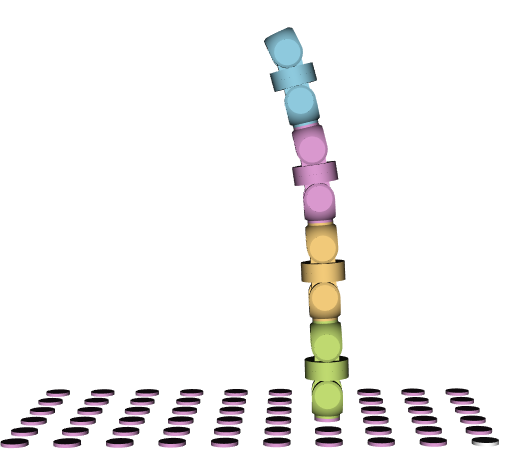
\includegraphics[width=0.19\textwidth]{sim2_1.png}
    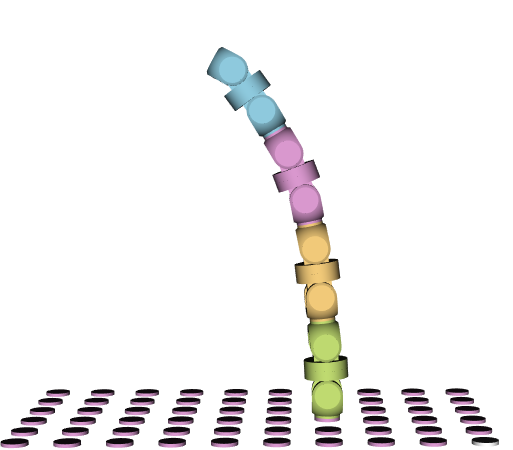
\includegraphics[width=0.19\textwidth]{sim2_2.png}
    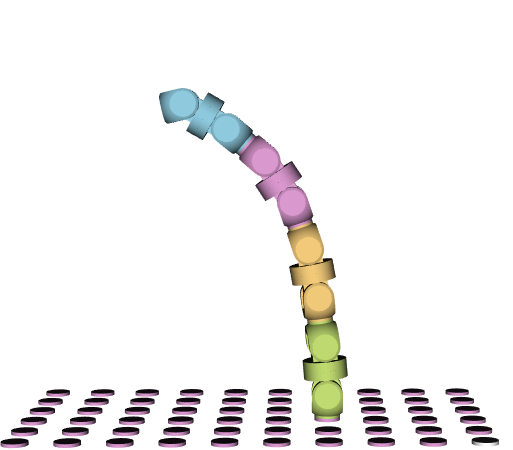
\includegraphics[width=0.19\textwidth]{sim2_3.png}
    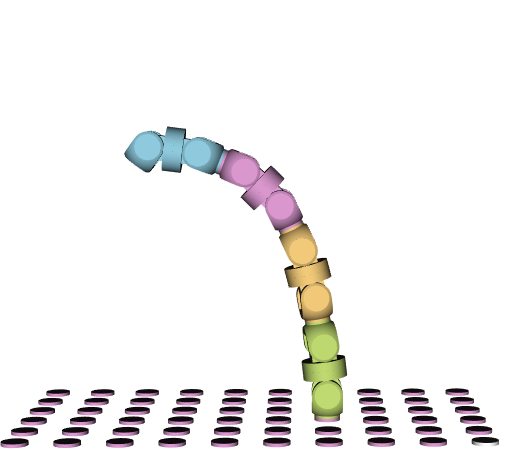
\includegraphics[width=0.19\textwidth]{sim2_4.png}
    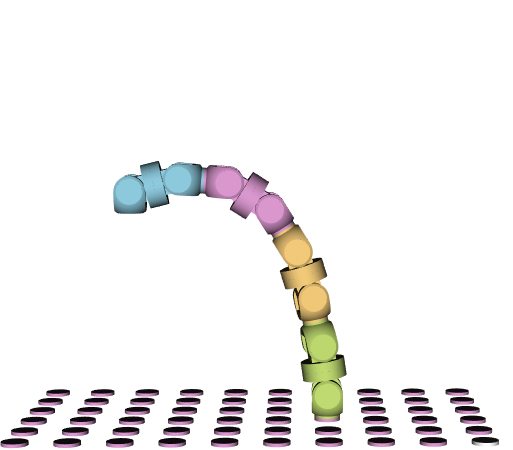
\includegraphics[width=0.19\textwidth]{sim2_5.png}
  \end{minipage}
  \caption{Our algorithm in a space with no obstacles, extended with trajectory shortcutting.}\label{fig:sim2}
\end{figure}

\clearpage

\section{A more efficient representation of space}

The algorithm is almost complete, but there is an issue we haven't addressed yet: usage of the grid to represent space.

The first issue with this representation is inefficiency: even if a segment is free from obstacles, we represent it with a regularly spaced out grid, wasting memory and making our shortest path algorithm slower and harder to scale to larger manipulators.

The second issue comes in the form of edge cases that are difficult to represent. If there are any obstacles smaller than the spacing of the grid, the algorithm can find paths that cause a collision. On the other hand, if there are large obstacles with small holes, the grid may not  find paths through the holes at all.

As inspiration for how to represent the space, we can think back to visibility graphs~\ref{fig:vis}. However, as established earlier, we don't want to use the edges of objects as vertices.

\begin{wrapfigure}{r}{0.4\textwidth}
  \centering
  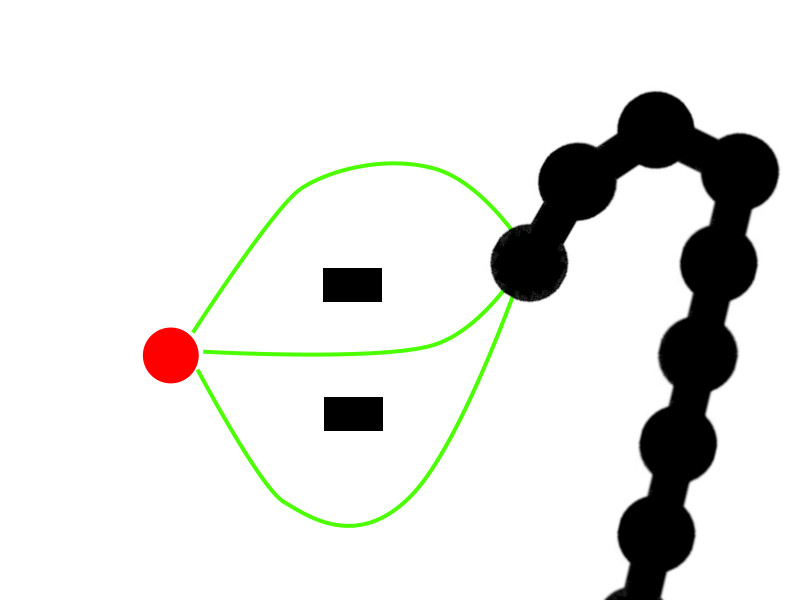
\includegraphics[width=0.4\textwidth]{obstacle_paths.png}
  \caption{3 relevant paths around a pair of obstacles.}
\end{wrapfigure}

Imagine a simple case of a manipulator trying to reach a target behind a pair of obstacles. The manipulator may either choose to go between them, around them from one side, or around them from the other. Therefore, for the purposes of representing this space, a simple graph is sufficient, instead of a complete grid. This graph has a vertex at the current \textit{end effector} position, a vertex at the target position, and 3 vertices surrounding the obstacles; one above, one below, and one between them. The 3 vertices need to be connected to both the initial and target positions.

In 3 dimensions, building such a graph is a bit more complex. Even so, we can define general directions obstacles the path can lead around. We can borrow the idea from visibility graphs: for every pair of obstacles that can see each other, an interesting point on the graph is the point halfway between them\footnote{Unless the obstacles are so close to each other that the joints of the manipulator cannot fit between them. Then, it makes no sense to consider the vertex.}.

Finding points between obstacles alone is not sufficient to represent all interesting paths -- we also want to look for paths that go around all the obstacles. Therefore, for the purposes of the algorithm, virtual obstacles are added at the edges of the manipulator's reach. Connecting these edges with nearby obstacles returns paths that lead around them, if they are within the manipulator's reach.

\begin{figure}
    \centering
    \begin{subfigure}{.45\textwidth}
      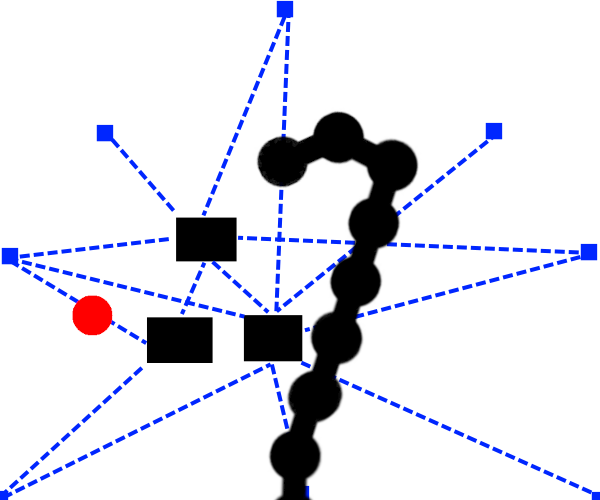
\includegraphics[width=0.99\textwidth]{ctrlgen_1_1.png}
      \caption{Virtual obstacles are created at the edges of the manipulator's reach, and all obstacles are connected (dark blue lines).}
    \end{subfigure}
    \begin{subfigure}{0.45\textwidth}
      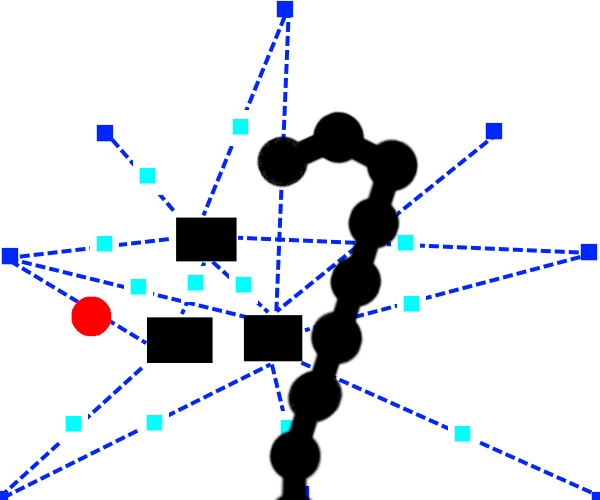
\includegraphics[width=0.99\textwidth]{ctrlgen_1_2.png}
      \caption{Points in between the obstacles become vertices of the graph (light blue squares).}
    \end{subfigure}

    \begin{subfigure}{.45\textwidth}
      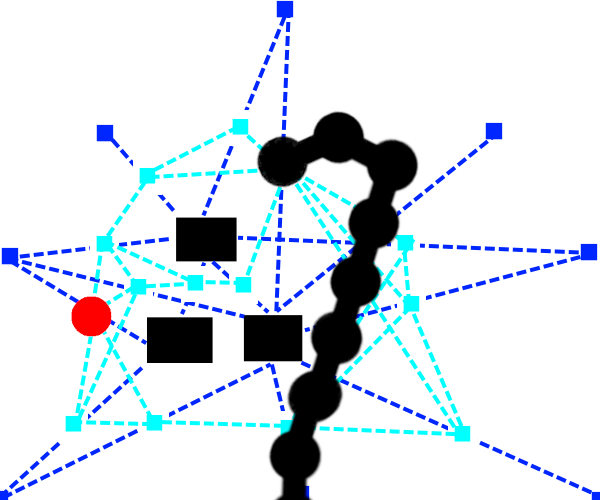
\includegraphics[width=0.99\textwidth]{ctrlgen_1_3.png}
      \caption{Vertices that see each other are connected with edges (light blue lines).}
    \end{subfigure}
    \begin{subfigure}{0.45\textwidth}
      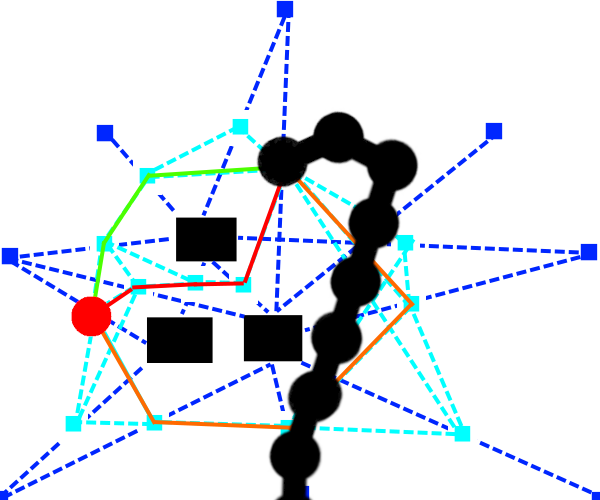
\includegraphics[width=0.99\textwidth]{ctrlgen_1_4.png}
      \caption{Example paths to the target in the created graph.}
    \end{subfigure}
    \caption{Illustration of how the graph representing the space is created and used to find a path to the target.}\label{fig:ctrlgen}
  \end{figure}

Just like visibility graphs, the vertices we create between obstacles are connected with an edge if they see each other, i.e.\ there are no obstacles between them.

The implementation of two points being visible to each other can be done trivially with the use of our built AABB. We define a line segment that leads from one obstacle to the other, and if it collides with any other object, the objects are not connected. The formula for line-sphere intersection is derived from the respective object equations; the slabs raycasting method~\cite{slabs} is used for detecting line-box intersection within the AABB.

The amount of vertices in a graph created this way can be bound by $\mathcal{O}(n^2)$ with respect to the number of obstacles -- at most there will be a vertex between each pair, and the number of virtual obstacles at the edges is constant. Unlike the grid approach and sampling based approaches, we are only paying a higher price for finding a path with an increasing number of obstacles, and are mostly unaffected when the workspace of the manipulator increases. This way of representing the workspace within the algorithm is particularly efficient for static manipulators in mostly unchanging environments but multiple consequent targets. Rather than building the whole graph every time we need to find a target, it is sufficient to update the source and target vertices, while the remainder of the graph stays the same.

Of course, there is a reason why we've discussed the grid based approach for so long: apart from the graph we are operating on, the rest of the algorithm remains the same.
The main takeaway from our grid based approach is that we want to assign a higher cost to vertices close to obstacles; this holds for our new graph as well. Each edge between vertices is assigned a cost based on the distance of the points to reflect the actual distance that needs to be traversed, while each vertex is assigned an additional cost for traversing over it based on how far it is from the surrounding obstacles.

When creating the vertices, we know how far apart the obstacles it was created between are. This directly gives us a way of assigning costs, since a path that leads closely between obstacles is higher-risk, while a path in some open space is safer. Therefore, we make the weights inversely proportional to the distance between the two objects.

Just like in the grid-based approach, we want to interpolate the found positions with a B-spline. Unlike the grid-based approach, the vertices are not spaced out evenly, and we want to use NURBS to extend each vertex with a weight. Recall that in a NURBS curve, each control point is associated with an additional weight, which determines how much it will affect the curve in its vicinity: a higher weight leads to paths closer to the point.

\begin{figure}
  \centering
  \begin{subfigure}{.45\textwidth}
    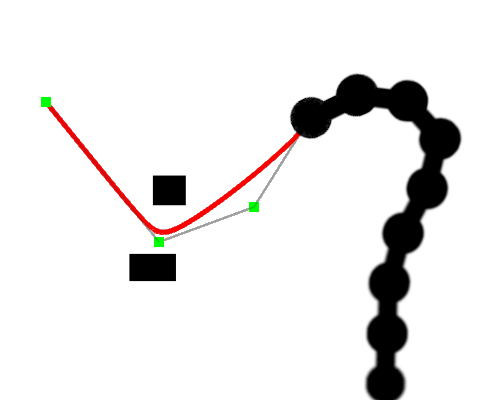
\includegraphics[width=0.99\textwidth]{nurbs_close.png}
    \caption{The control point between obstacles has a high weight, so that the manipulator follows the path closely and fits between them.}
  \end{subfigure}
  \begin{subfigure}{0.45\textwidth}
    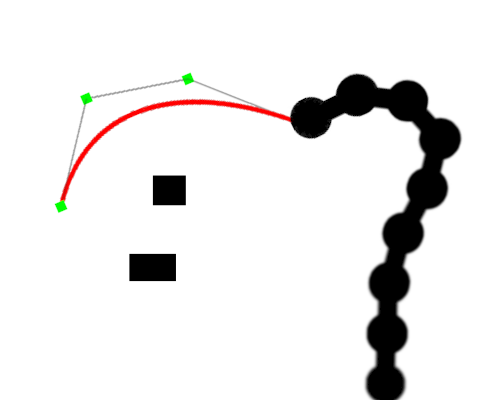
\includegraphics[width=0.99\textwidth]{nurbs_far.png}
    \caption{The control points created in the open space between the edges and obstacles have a low weight and only need to be followed loosely.}
  \end{subfigure}
  \caption{Illustration of how weights of vertices affect the resulting path.}\label{fig:nurb_paths}
\end{figure}

The weight associated with a given vertex directly translates to the weight of the resulting NURBS curve. Since each weight represents how close the surrounding obstacles are, it also represents how close to the point we need the curve to be in order to avoid them. When the obstacles are close, we need the weight of the NURBS control point to be high in order to fit in small passages. On the other hand, if the point is in an open space, we only need to approach it loosely, and trying to go to the middle of the open space could lead to unnecessary motion (see Figure~\ref{fig:nurb_paths}).

\section{The final algorithm}

Finally, we have a complete algorithm for trajectory generation of high DoF robotic arms:

\begin{enumerate}
\item The environment within which the manipulator exists is loaded, and a kinematic model of the manipulator is created.
\item An AABB tree for collision checking is created. The obstacles and joints are approximated via spheres and inserted into the tree.
\item A graph is generated by using the space between obstacles as vertices, and connecting vertices with an edge if the direct line between them is unobstructed by obstacles.
\item The shortest path on the weighted graph between the initial position of the \textit{end effector} and the target is found.
\item The found path is smoothed out by interpolating the vertices with a NURBS curve.
\item The path is sampled at discrete points, and an extension of FABRIK is used to compute the joint parameters needed to reach each of the points.
\item If FABRIK fails to find viable positions on the path, the path is evaluated as unsuccessful. The algorithm increases the cost of the vertices on the path, falls back to step 4 and tries to find a different path in the modified graph.
\item If FABRIK finds viable positions on the path, use a shortcutting algorithm to post-process the path and minimize unnecessary movement.
\end{enumerate}

After finding all the intermediate positions, the motion can be realised by moving the manipulator's joints.

To analyze the complexity of our new algorithm, we need to look at the individual components and analyze the work done in them. The two parameters that influence the complexity are the number of joints, which we can denote with $j$, and the number of obstacles, which we can denote with $n$.

The first operation that takes place is building the AABB tree. This process consists of inserting each joint and obstacle into the AABB, meaning $\mathcal{O}(j + n)$ insertions. As discussed earlier, no guarantees on the depth of the tree are given, which leads to a linear worst-case complexity of having to make a number of comparisons equal to the number of already inserted objects. Therefore, we can only bound the building of the tree by $\mathcal{O}({(j+n)}^2)$, although the average complexity will be much lower.

To create the graph of vertices between obstacles, the path between each pair of obstacles is checked, bound by $\mathcal{O}(n^2 (j+n))$ due to the $\mathcal{O}(j+n)$ collision checking within the AABB. The upper limit on th enumber of vertices is $n^2$, therefore the creation of edges between each pair can be bound by $\mathcal{O}(n^4 (j+n))$.

Finding the shortest path is done with Djikstra's algorithm, using a priority queue implemented with a standard binary heap. Since the complexity of Djikstra is $\mathcal{O}((|V|+|E|) \log{|V|})$, we can bound it with respect to the number of obstacles with $\mathcal{O}(n^4 \log{n})$.

Since we are discretizing the path at constant intervals, the number of times we compute FABRIK on each path depends on the path's length. In the case of RoFI manipulators, the distance between all the joints is constant; hence, we can get a rough estimation of the maximal length of the path with respect to the number of joints. Since the maximal reach of the manipulator in one direction is bound by $\mathcal{O}(j)$ and it can move in 3 dimensions, the maximal length of the path, as well as the targets on it, is $\mathcal{O}(j^3)$.

A single FABRIK iteration is linear to the number of joints. At each joint, we find the right position for the current joint ($\mathcal{O}(1)$), check if the current joint collides with any obstacles ($\mathcal{O}(j+n)$) and recompute the transformation matrices of all the following joints ($\mathcal{O}(j)$). FABRIK stops when the target is reached, when it gets stuck, or a constant iteration limit is hit without reaching the target. Therefore, the upper bound on the complexity of FABRIK for a single target is $\mathcal{O}(j^2(j+n))$.

If the first path is evaluated as unsuccessful, we try different paths, but the total number of paths we explore can be bound by a small constant. Therefore, the total complexity of the algorithm is $\mathcal{O}(n^4(j+n)+j^5(j+n)) = \mathcal{O}(n^5+j^6)$. Although this complexity may seem quite high, note that we've used very rough estimates and each individual operation is very cheap. Multplying $4 \times 4$ matrices and doing simple number comparisons while collision checking are operations that are quite trivial and heavily optimized. And since the entire algorithm is clearly polynomial with respect to the number of joints, we've achieved the goal of making it scalable; unlike the state of the art approaches exponential to the number of joints.
